\documentclass{standalone}
\usepackage{tikz,pgfplots}
\usepackage{amsmath}
\usetikzlibrary{arrows,positioning}

\usepackage{amssymb}
%\usepackage[latin1]{inputenc}
\usepackage{algpseudocode}
\usepackage{algorithm}
\usepackage{pgfplots,tikz,standalone}
\usepackage{mathtools,subcaption,enumitem}
\usepackage{multirow}
\usepackage{color}
%% The amsthm package provides extended theorem environments
\usepackage{amsthm}
\usepackage{url}
% \usepackage[dvips]{graphicx}
%\usetikzlibrary{arrows,positioning}
%\usepackage{subfig}

\usetikzlibrary{calc,patterns,angles,quotes,babel}

\usetikzlibrary{external}
\tikzset{external/system call={pdflatex \tikzexternalcheckshellescape 
		-halt-on-error
		-interaction=batchmode 
		-jobname "\image" "\texsource"
		&& pdftops -eps "\image.pdf"}}
\tikzexternalize

\def\uW{\mathit{\mu W}}

\begin{document}
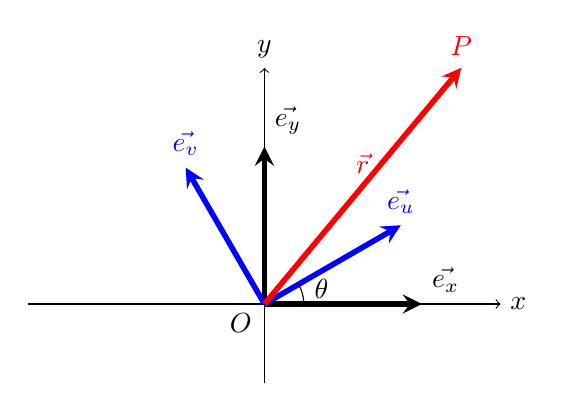
\begin{tikzpicture}

\coordinate (a) at (0,0) node[anchor=south,below,xshift=-0.3cm]{$O$};
\coordinate (b) at (0.866,0.5);
\coordinate (c) at (0.866,0);

\draw[thin,gray!40] (-3,-1) (3,3);
\draw[->] (-3,0)--(3,0) node[right]{$x$};
\draw[->] (0,-1)--(0,3) node[above]{$y$};
\draw[line width=2pt,black,-stealth](0,0)--(2,0) node[anchor=south,xshift=0.3cm]{$\vec{e_x}$};
\draw[line width=2pt,black,-stealth](0,0)--(0,2) node[anchor=south,xshift=0.3cm]{$\vec{e_y}$};

%\draw[red] node[]{$P$}

\draw[line width=2pt,blue,-stealth](0,0)--(1.732,1) node[anchor=south]{$\vec{e_u}$};
\draw[line width=2pt,blue,-stealth](0,0)--(-1,1.732) node[anchor=south]{$\vec{e_v}$};

\draw[line width=2pt,red,-stealth](0,0)--(2.5,3) node[anchor=south,above, midway]{$\vec{r}$} node[anchor=south]{$P$};

%\path[clip] (0.866,0.5) -- (0,0) -- (0.866,0) -- cycle;
%\node[circle,draw=black,minimum size=40pt] at (0,0) (circ) {};
%\draw[blue] (1cm,0cm) arc (90:125:0.5cm);

%  \draw
%(3,-1) coordinate (a) node[right] {a}
%-- (0,0) coordinate (b) node[left] {b}
%-- (2,2) coordinate (c) node[above right] {c}
%pic["$\alpha$",draw=orange,<->,angle eccentricity=1.2,angle radius=1cm] {angle=a--b--c};

\pic [draw, -, "$\theta$", angle eccentricity=1.5] {angle = c--a--b};


%\draw[line width=2pt,blue,-stealth](0,0)--(-0.5,$\sqrt{3}/2$) node[anchor=south]{$\vec{e_v}$};

\end{tikzpicture}
\end{document}

